\documentclass[10pt]{article}
\usepackage[utf8]{inputenc}
\usepackage[T1]{fontenc}
\usepackage{amsmath}
\usepackage{amsfonts}
\usepackage{amssymb}
\usepackage[version=4]{mhchem}
\usepackage{stmaryrd}
\usepackage{graphicx}
\usepackage[export]{adjustbox}
\graphicspath{ {./images/} }

\begin{document}
\begin{enumerate}
  \item Which of the following rational functions have a horizontal asymptote?\\
I. $f(x)=\frac{3 x^{2}+x-1}{x^{2}+4}$\\
II. $g(x)=\frac{(x+1)(2 x-3)^{2}}{(5 x-7)^{2}}$\\
III. $h(x)=\frac{x-4}{x^{3}+x^{2}-6}$\\
(A) I only\\
(B) I and II only\\
(C) I and III only\\
(D) I, II, and III
  \item The graph of the rational function h has a horizontal asymptote of $y=-3$. Which of the following could be an expression for $h(x)$ ?\\
(A) $\frac{x^{2}-4 x+7}{-3 x^{2}+5}$\\
(B) $\frac{3 x^{2}-5 x-2}{x^{2}-x+1}$\\
(C) $\frac{-3 x^{3}+x-2}{x^{2}+5 x-6}$\\
(D) $\frac{-6 x^{3}+7 x^{2}-12}{2 x^{3}+11}$
\end{enumerate}

The graph of the rational function $f$ is shown below. Use the graph of $f$ to answer the following questions:\\
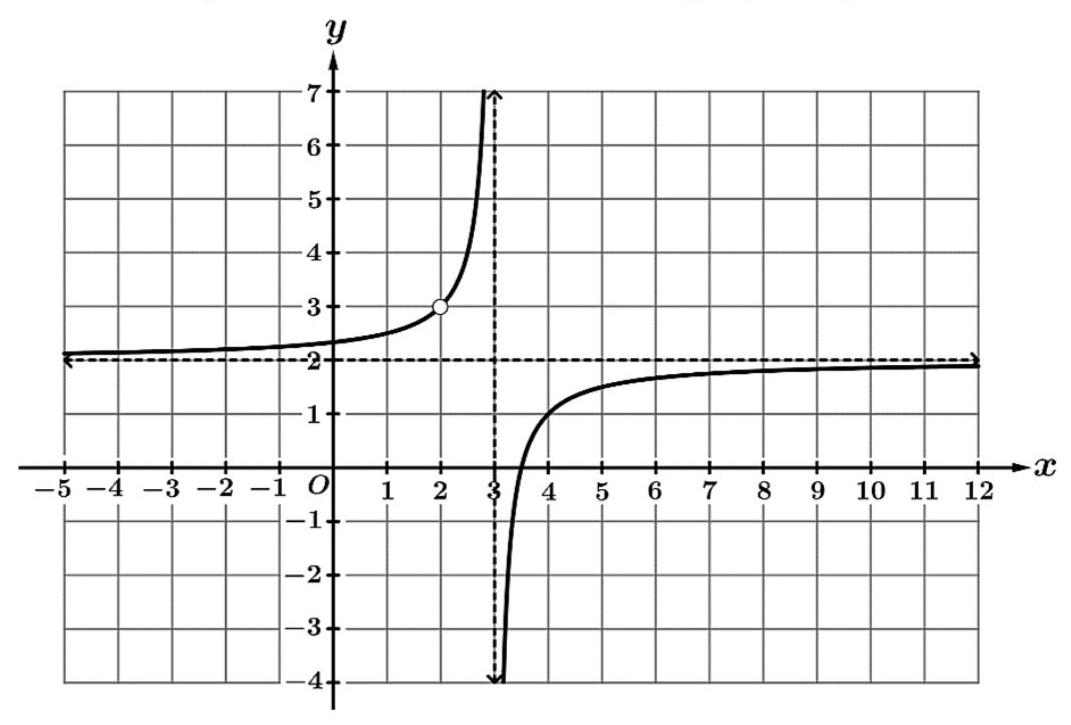
\includegraphics[max width=\textwidth, alt={}, center]{bb0c961a-4a4c-4f4a-bec0-1e84a1708d3c-01_725_1071_1237_575}\\
3. $\lim _{x \rightarrow 3^{+}} f(x)=$\\
(A) 2\\
(B) 3\\
(C) $-\infty$\\
(D) $\infty$\\
4. $\lim _{x \rightarrow-\infty} f(x)=$\\
(A) 2\\
(B) 3\\
(C) $-\infty$\\
(D) $\infty$\\
5. $\lim _{x \rightarrow 2^{-}} f(x)=$\\
(A) 2\\
(B) 3\\
(C) $-\infty$\\
(D) $\infty$\\
6. Let $g(x)=\frac{(x-2)^{2}(x+3)^{3}(x-4)^{2}}{(x-2)^{3}(x+3)^{2}}$. The graph of $g$ has a zeros at which of the following values of $x$ ?\\
(A) $x=4$ only\\
(B) $x=4$ and $x=-3$ only\\
(C) $x=2$ and $x=-3$ only\\
(D) $x=4, x=2$, and $x=-3$\\
7. The graph of the rational function $h$ is shown below. Which of the following could be the expression for $h$ ?\\
(A) $\frac{(x-3)}{(x-3)(x-1)}$\\
(B) $\frac{(x+1)(x-3)}{(x-3)(x-1)}$\\
(C) $\frac{(x+1)(x-1)}{(x-3)(x-1)}$\\
(D) $\frac{(x-1)(x-3)}{(x-3)(x+1)}$\\
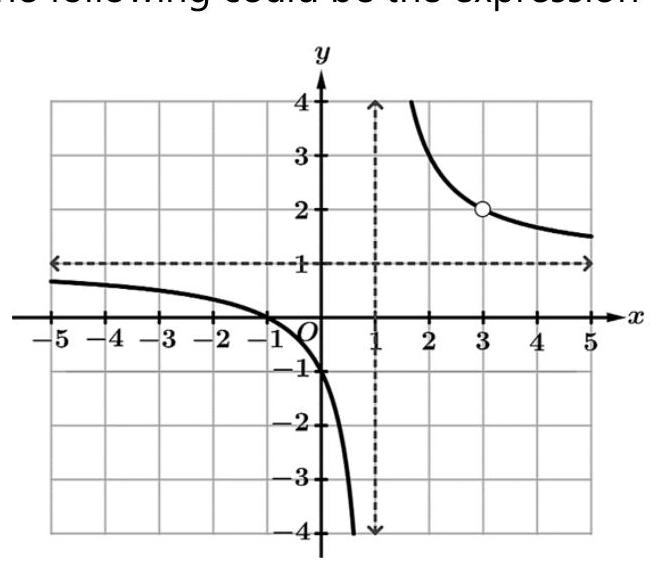
\includegraphics[max width=\textwidth, alt={}, center]{bb0c961a-4a4c-4f4a-bec0-1e84a1708d3c-02_568_654_818_1261}\\
8. If $\frac{12-6 x}{(x-1)(x+2)}=\frac{A}{x-1}+\frac{B}{x+2^{\prime}}$, what is the value of $A$ ?\\
(A) 2\\
(B) 8\\
(C) -2\\
(D) -8\\
9. A rational function $r$ is given by $r(x)=\frac{x-2}{x+3}$. What are all intervals on which $r(x)>0$ ?\\
(A) $(-3,2)$\\
B) $(2, \infty)$\\
(C) $(-\infty,-3) \cup(2, \infty)$\\
(D) $(-\infty,-2) \cup(3, \infty)$\\
10. Let $h(x)=\frac{(x-2)(x+1)^{2}}{(x+1)(x-2)^{2}}$. Which of the following statements about the graph of $h$ is correct?\\
(A) The graph of $h$ has one hole and one vertical asymptote.\\
(B) The graph of $h$ has two holes and no vertical asymptotes.\\
(C) The graph of $h$ has no holes and two vertical asymptotes.\\
(D) The graph of $h$ has one hole and two vertical asymptotes.\\
11. The graph of the rational function $f$ has a hole at $x=5$ and a vertical asymptote at $x=-3$. Which of the following could be the expression for $f$ ?\\
(A) $\frac{(x-5)(x+2)}{(x-5)(x+3)}$\\
(B) $\frac{(x+2)(x+3)}{(x-5)(x+3)}$\\
(C) $\frac{(x-5)(x+3)}{(x-5)(x+2)}$\\
(D) $\frac{(x+5)(x+2)}{(x+5)(x-3)}$\\
12. Let $h(x)=\frac{x^{3}+x^{2}-20 x}{x^{2}-8 x+16}$. Which of the following statements about the graph of $h$ is correct when $x=4$ ?\\
(A) The graph of $h$ only has a zero when $x=4$.\\
(B) The graph of $h$ only has a hole when $x=4$.\\
(C) The graph of $h$ only has a vertical asymptote when $x=4$.\\
(D) The graph of $h$ has both a zero and a vertical asymptote when $x=4$.

Use the function $r(x)=\frac{2 x^{3}-6 x+4}{4 x^{3}+12 x^{2}-16}$ to answer the questions below.\\
a) Factor $r(x)$ and write it in a simplified form. Be sure to include domain restrictions (3 points)\\
b) Find the following key features of $r(x)$ (6 points). Then, sketch $r(x)$ on the axes provided (1 point)

\begin{center}
\begin{tabular}{|c|l|}
\hline
Domain &  \\
\hline
Vertical &  \\
Asymptote(s) &  \\
\hline
\begin{tabular}{c}
Horizontal \\
Asymptote(s) \\
\end{tabular} &  \\
\hline
Y-intercept(s) &  \\
\hline
X-intercept(s) &  \\
\hline
Hole(s) &  \\
\hline
\end{tabular}
\end{center}

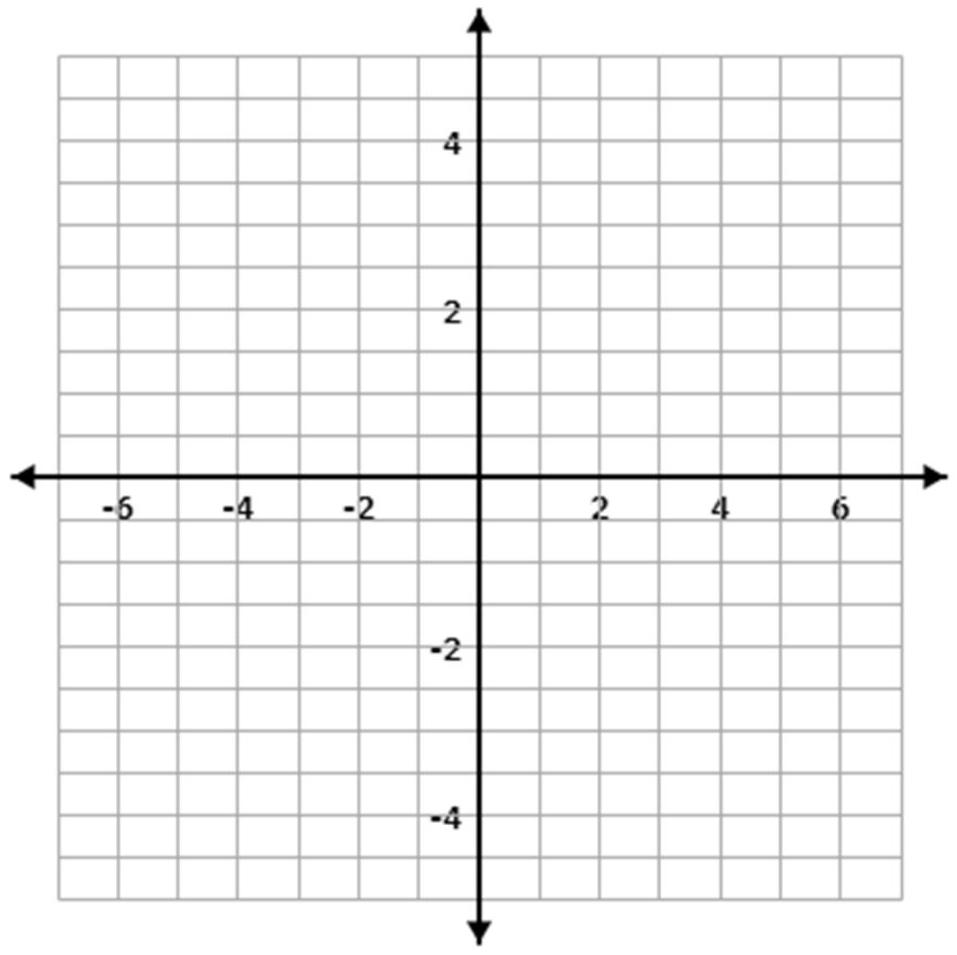
\includegraphics[max width=\textwidth, alt={}, center]{bb0c961a-4a4c-4f4a-bec0-1e84a1708d3c-04_955_957_1003_964}\\
c) Write the end behavior of $r(x)$ as $x$ increases without bound as a limit statement (2 points)\\
d) Evaluate the 2 limits shown below (1 point each)

$$
\lim _{x \rightarrow-2^{+}} r(x)=\quad \lim _{x \rightarrow 1^{+}} r(x)=
$$

Simplify the expression (3 points)

$$
\frac{\frac{8 x}{x^{2}-1}}{\frac{10 x}{x+1}}
$$

Simplify the expression (3 points)

$$
\frac{4+\frac{1}{x^{2}}}{3-\frac{1}{x^{2}}}
$$

Find all real values of $x$ that satisfy the equation. Identify all algebraic solutions and indicate extraneous solutions by striking through them. (4 points)

$$
\frac{1}{x-4}-\frac{5}{x+2}=\frac{6}{x^{2}-2 x-8}
$$

Find all real values of $x$ that satisfy the equation. Identify all algebraic solutions and indicate extraneous solutions by striking through them. (5 points)

$$
\frac{2 x^{2}+5 x-5}{x-x^{2}}+\frac{1+x^{-1}}{1-x^{-1}}=\frac{1-x}{-x}
$$

\begin{enumerate}
  \item The graph of the rational function h has a horizontal asymptote of $y=-3$. Which of the following could be an expression for $h(x)$ ?\\
(A) $\frac{x^{2}-4 x+7}{-3 x^{2}+5}$\\
(B) $\frac{3 x^{2}-5 x-2}{x^{2}-x+1}$\\
(C) $\frac{-3 x^{3}+x-2}{x^{2}+5 x-6}$\\
(D) $\frac{-6 x^{3}+7 x^{2}-12}{2 x^{3}+11}$
  \item Which of the following rational functions have a horizontal asymptote?\\
I. $f(x)=\frac{3 x^{2}+x-1}{x^{2}+4}$\\
II. $g(x)=\frac{(x+1)(2 x-3)^{2}}{(5 x-7)^{2}}$\\
III. $h(x)=\frac{x-4}{x^{3}+x^{2}-6}$\\
(A) I only\\
(B) I and II only\\
(C) I and III only\\
(D) I, II, and III
\end{enumerate}

The graph of the rational function $f$ is shown below. Use the graph of $f$ to answer the following questions:\\
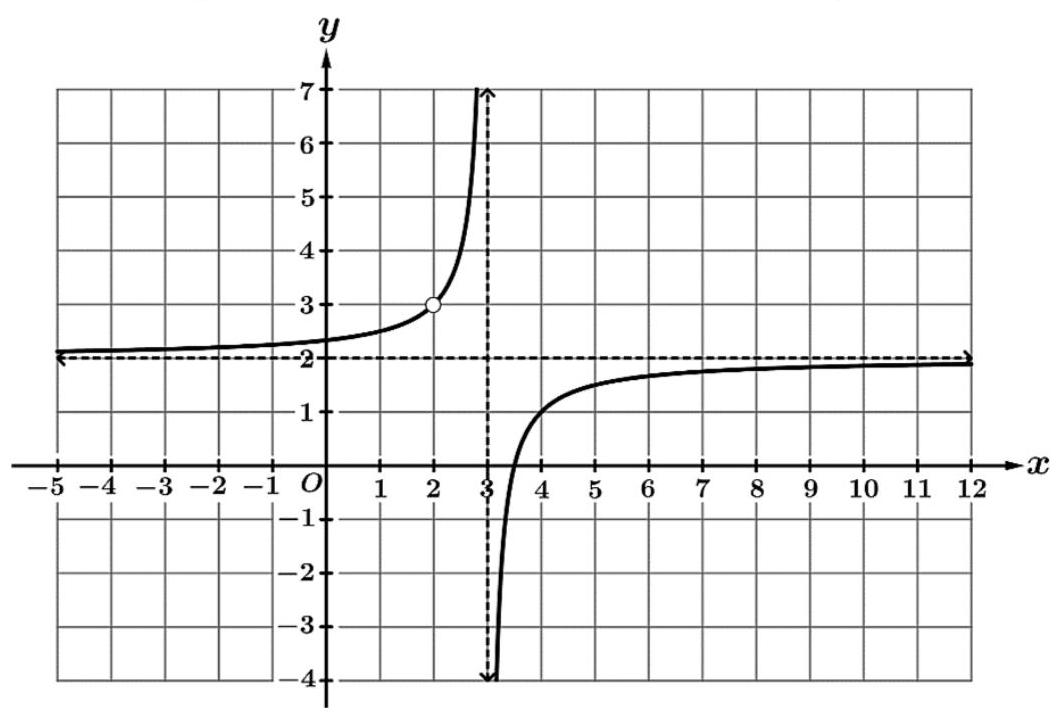
\includegraphics[max width=\textwidth, alt={}, center]{bb0c961a-4a4c-4f4a-bec0-1e84a1708d3c-07_719_1062_1239_582}\\
3. $\lim _{x \rightarrow 2^{-}} f(x)=$\\
(A) 2\\
(B) 3\\
(C) $-\infty$\\
(D) $\infty$\\
4. $\lim _{x \rightarrow-\infty} f(x)=$\\
(A) 2\\
(B) 3\\
(C) $-\infty$\\
(D) $\infty$\\
5. $\lim _{x \rightarrow 3^{+}} f(x)=$\\
(A) 2\\
(B) 3\\
(C) $-\infty$\\
(D) $\infty$\\
6. A rational function $r$ is given by $r(x)=\frac{x-2}{x+3}$. What are all intervals on which $r(x)>0$ ?\\
(A) $(-3,2)$\\
B) $(2, \infty)$\\
(C) $(-\infty,-3) \cup(2, \infty)$\\
(D) $(-\infty,-2) \cup(3, \infty)$\\
7. If $\frac{12-6 x}{(x-1)(x+2)}=\frac{A}{x-1}+\frac{B}{x+2}$, what is the value of $B$ ?\\
(A) 2\\
(B) 8\\
(C) -2\\
(D) -8\\
8. The graph of the rational function $h$ is shown below. Which of the following could be the expression for $h$ ?\\
(A) $\frac{(x-3)}{(x-3)(x-1)}$\\
(B) $\frac{(x+1)(x-3)}{(x-3)(x-1)}$\\
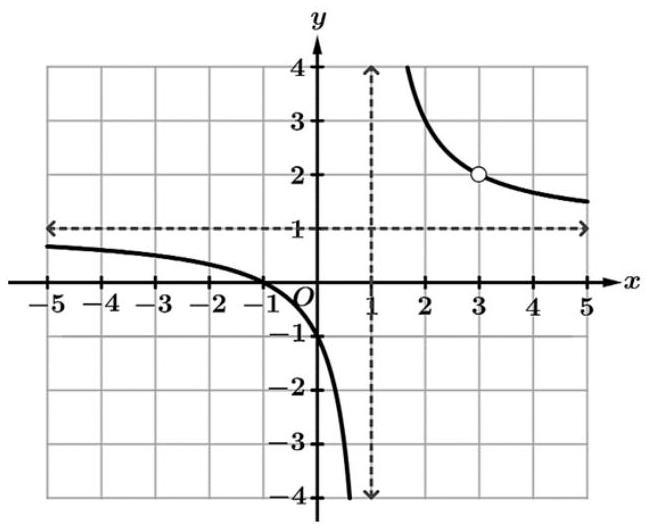
\includegraphics[max width=\textwidth, alt={}, center]{bb0c961a-4a4c-4f4a-bec0-1e84a1708d3c-08_531_654_1491_1291}\\
9. Let $g(x)=\frac{(x-2)^{2}(x+3)^{3}(x-4)^{2}}{(x-2)^{3}(x+3)^{2}}$. The graph of $g$ has a zeros at which of the following values of $x$ ?\\
(A) $x=4$ only\\
(B) $x=4$ and $x=-3$ only\\
(C) $x=2$ and $x=-3$ only\\
(D) $x=4, x=2$, and $x=-3$\\
10. Let $h(x)=\frac{x^{3}+x^{2}-20 x}{x^{2}-8 x+16}$. Which of the following statements about the graph of $h$ is correct when $x=4$ ?\\
(A) The graph of $h$ only has a zero when $x=4$.\\
(B) The graph of $h$ only has a hole when $x=4$.\\
(C) The graph of $h$ only has a vertical asymptote when $x=4$.\\
(D) The graph of $h$ has both a zero and a vertical asymptote when $x=4$.\\
11. The graph of the rational function $f$ has a hole at $x=5$ and a vertical asymptote at $x=-3$. Which of the following could be the expression for $f$ ?\\
(A) $\frac{(x-5)(x+2)}{(x-5)(x+3)}$\\
(B) $\frac{(x+2)(x+3)}{(x-5)(x+3)}$\\
(C) $\frac{(x-5)(x+3)}{(x-5)(x+2)}$\\
(D) $\frac{(x+5)(x+2)}{(x+5)(x-3)}$\\
12. Let $h(x)=\frac{(x-2)(x+1)^{2}}{(x+1)(x-2)^{2}}$. Which of the following statements about the graph of $h$ is correct?\\
(A) The graph of $h$ has one hole and one vertical asymptote.\\
(B) The graph of $h$ has two holes and no vertical asymptotes.\\
(C) The graph of $h$ has no holes and two vertical asymptotes.\\
(D) The graph of $h$ has one hole and two vertical asymptotes.

Use the function $r(x)=\frac{4 x^{3}+12 x^{2}-16}{2 x^{3}-6 x+4}$ to answer the questions below.\\
a) Factor $r(x)$ and write it in a simplified form. Be sure to include domain restrictions (3 points)\\
b) Find the following key features of $r(x)$ (6 points). Then, sketch $r(x)$ on the axes provided (1 point)

\begin{center}
\begin{tabular}{|c|l|}
\hline
Domain &  \\
\hline
Vertical &  \\
Asymptote(s) &  \\
\hline
Horizontal &  \\
Asymptote(s) &  \\
\hline
Y-intercept(s) &  \\
\hline
X-intercept(s) &  \\
\hline
Hole(s) &  \\
\hline
\end{tabular}
\end{center}

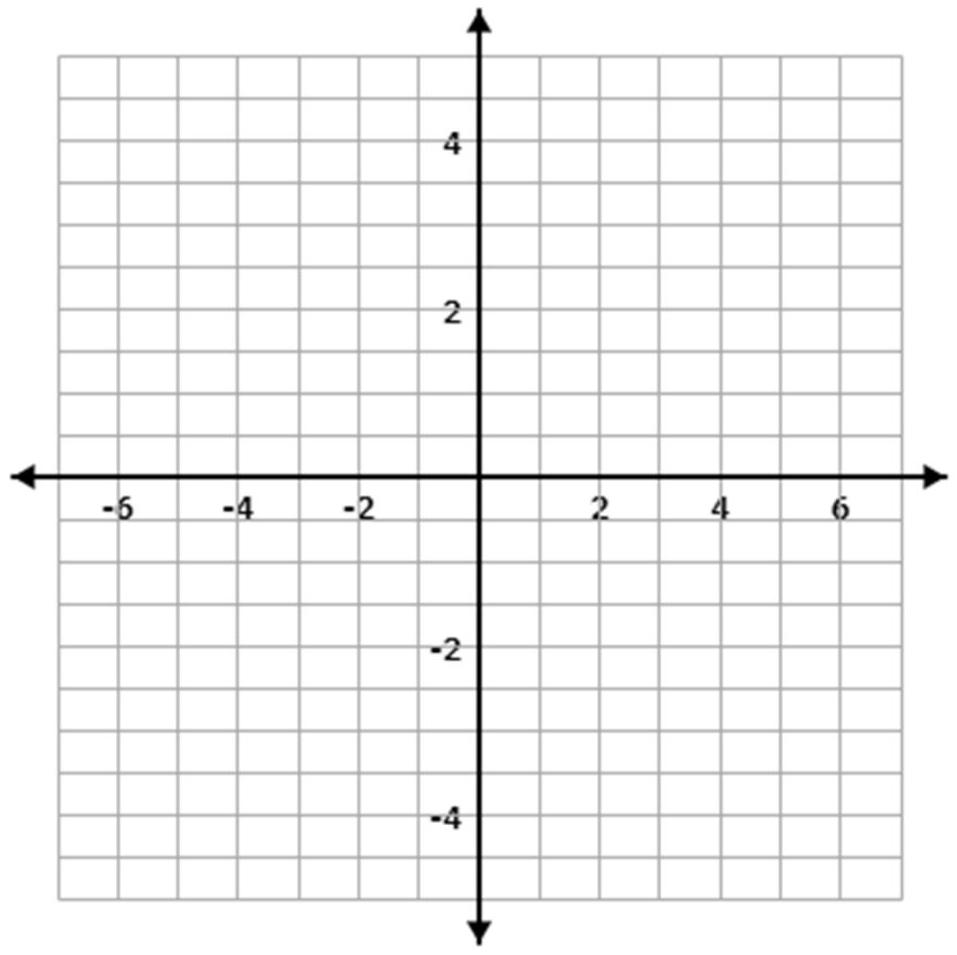
\includegraphics[max width=\textwidth, alt={}, center]{bb0c961a-4a4c-4f4a-bec0-1e84a1708d3c-10_955_957_1003_964}\\
c) Write the end behavior of $r(x)$ as $x$ increases without bound as a limit statement (2 points)\\
d) Evaluate the 2 limits shown below (1 point each)

$$
\lim _{x \rightarrow-2^{+}} r(x)=\quad \lim _{x \rightarrow 1^{+}} r(x)=
$$

Simplify the expression (3 points)

$$
\frac{\frac{x-2}{4 x}}{\frac{x^{2}-4 x+4}{12 x}}
$$

Simplify the expression (3 points)

$$
\frac{\frac{1}{x}+8}{4-\frac{1}{x}}
$$

Find all real values of $x$ that satisfy the equation. Identify all algebraic solutions and indicate extraneous solutions by striking through them. (4 points)

$$
\frac{1}{x-3}-\frac{2}{x+1}=\frac{8}{x^{2}-2 x-3}
$$

Find all real values of $x$ that satisfy the equation. Identify all algebraic solutions and indicate extraneous solutions by striking through them. (5 points)

$$
\frac{3 x^{2}+2 x-3}{x-x^{2}}+\frac{1+x^{-1}}{1-x^{-1}}=\frac{1-x}{-x}
$$

\begin{enumerate}
  \item The graph of the rational function $f$ has a hole at $x=5$ and a vertical asymptote at $x=-3$. Which of the following could be the expression for $f$ ?\\
(A) $\frac{(x-5)(x+2)}{(x-5)(x+3)}$\\
(B) $\frac{(x+2)(x+3)}{(x-5)(x+3)}$\\
(C) $\frac{(x-5)(x+3)}{(x-5)(x+2)}$\\
(D) $\frac{(x+5)(x+2)}{(x+5)(x-3)}$
  \item Let $h(x)=\frac{x^{3}+x^{2}-20 x}{x^{2}-8 x+16}$. Which of the following statements about the graph of $h$ is correct when $x=4$ ?\\
(A) The graph of $h$ only has a zero when $x=4$.\\
(B) The graph of $h$ only has a hole when $x=4$.\\
(C) The graph of $h$ only has a vertical asymptote when $x=4$.\\
(D) The graph of $h$ has both a zero and a vertical asymptote when $x=4$.
  \item Let $h(x)=\frac{(x-2)(x+1)^{2}}{(x+1)(x-2)^{2}}$. Which of the following statements about the graph of $h$ is correct?\\
(A) The graph of $h$ has one hole and one vertical asymptote.\\
(B) The graph of $h$ has two holes and no vertical asymptotes.\\
(C) The graph of $h$ has no holes and two vertical asymptotes.\\
(D) The graph of $h$ has one hole and two vertical asymptotes.
  \item The graph of the rational function $h$ is shown below. Which of the following could be the expression for $h$ ?\\
(A) $\frac{(x-3)}{(x-3)(x-1)}$\\
(B) $\frac{(x+1)(x-3)}{(x-3)(x-1)}$\\
(C) $\frac{(x+1)(x-1)}{(x-3)(x-1)}$\\
(D) $\frac{(x-1)(x-3)}{(x-3)(x+1)}$\\
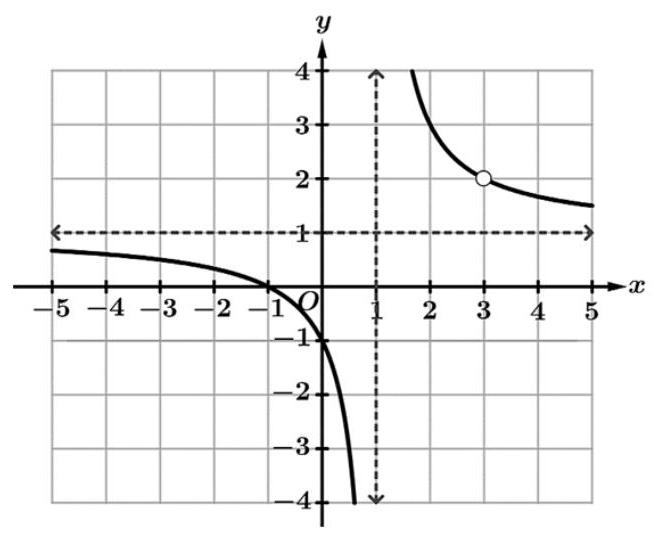
\includegraphics[max width=\textwidth, alt={}, center]{bb0c961a-4a4c-4f4a-bec0-1e84a1708d3c-14_539_660_216_1293}
  \item Let $g(x)=\frac{(x-2)^{2}(x+3)^{3}(x-4)^{2}}{(x-2)^{3}(x+3)^{2}}$. The graph of $g$ has a zeros at which of the following values of $x$ ?\\
(A) $x=4$ only\\
(B) $x=4$ and $x=-3$ only\\
(C) $x=2$ and $x=-3$ only\\
(D) $x=4, x=2$, and $x=-3$
  \item A rational function $r$ is given by $r(x)=\frac{x-2}{x+3}$. What are all intervals on which $r(x)>0$ ?\\
(A) $(-3,2)$\\
B) $(2, \infty)$\\
(C) $(-\infty,-3) \cup(2, \infty)$\\
(D) $(-\infty,-2) \cup(3, \infty)$
  \item If $\frac{12-6 x}{(x-1)(x+2)}=\frac{A}{x+2}+\frac{B}{x-1}$, what is the value of $A$ ?\\
(A) 2\\
(B) 8\\
(C) -2\\
(D) -8
\end{enumerate}

The graph of the rational function $f$ is shown below. Use the graph of $f$ to answer the following questions:\\
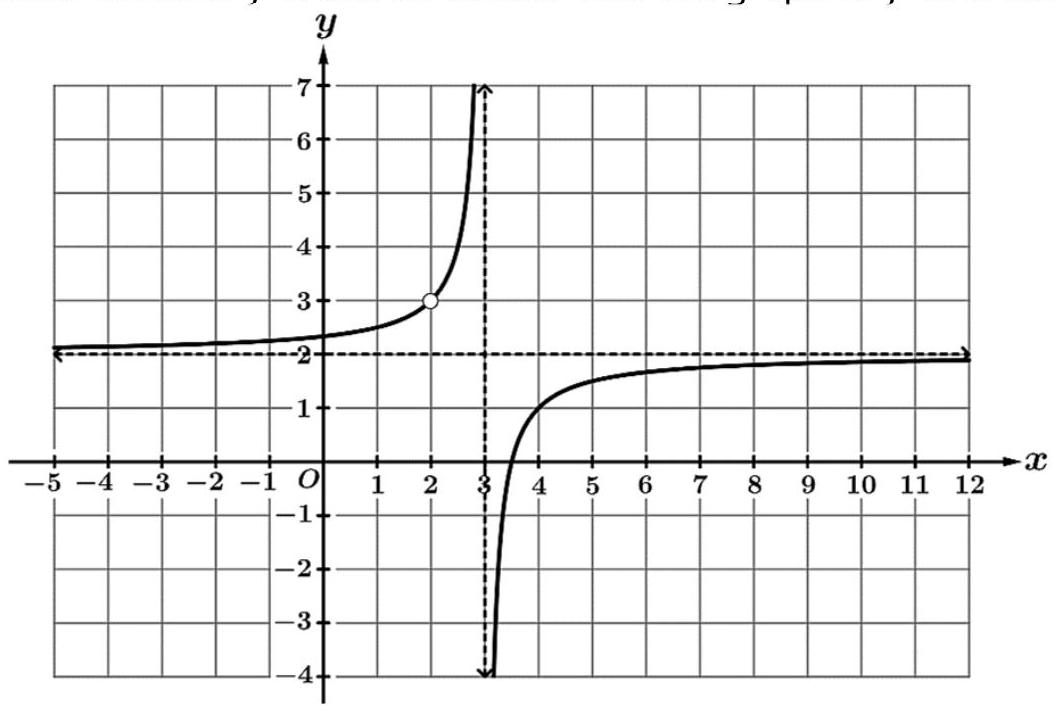
\includegraphics[max width=\textwidth, alt={}, center]{bb0c961a-4a4c-4f4a-bec0-1e84a1708d3c-15_717_1060_182_532}\\
8. $\lim _{x \rightarrow 2^{-}} f(x)=$\\
(A) 2\\
(B) 3\\
(C) $-\infty$\\
(D) $\infty$\\
9. $\lim _{x \rightarrow-\infty} f(x)=$\\
(A) 2\\
(B) 3\\
(C) $-\infty$\\
(D) $\infty$\\
10. $\lim _{x \rightarrow 3^{+}} f(x)=$\\
(A) 2\\
(B) 3\\
(C) $-\infty$\\
(D) $\infty$\\
11. The graph of the rational function h has a horizontal asymptote of $y=-3$. Which of the following could be an expression for $h(x)$ ?\\
(A) $\frac{x^{2}-4 x+7}{-3 x^{2}+5}$\\
(B) $\frac{3 x^{2}-5 x-2}{x^{2}-x+1}$\\
(C) $\frac{-3 x^{3}+x-2}{x^{2}+5 x-6}$\\
(D) $\frac{-6 x^{3}+7 x^{2}-12}{2 x^{3}+11}$\\
12. Which of the following rational functions have a horizontal asymptote?\\
I. $f(x)=\frac{3 x^{2}+x-1}{x^{2}+4}$\\
II. $g(x)=\frac{(x+1)(2 x-3)^{2}}{(5 x-7)^{2}}$\\
III. $h(x)=\frac{x-4}{x^{3}+x^{2}-6}$\\
(A) I only\\
(B) I and II only\\
(C) I and III only\\
(D) I, II, and III

Use the function $r(x)=\frac{2 x^{3}+6 x^{2}-8}{4 x^{3}-12 x+8}$ to answer the questions below.\\
a) Factor $r(x)$ and write it in a simplified form. Be sure to include domain restrictions (3 points)\\
b) Find the following key features of $r(x)$ (6 points). Then, sketch $r(x)$ on the axes provided (1 point)

\begin{center}
\begin{tabular}{|c|l|}
\hline
Domain &  \\
\hline
Vertical &  \\
Asymptote(s) &  \\
\hline
Horizontal &  \\
Asymptote(s) &  \\
\hline
Y-intercept(s) &  \\
\hline
X-intercept(s) &  \\
\hline
Hole(s) &  \\
\hline
\end{tabular}
\end{center}

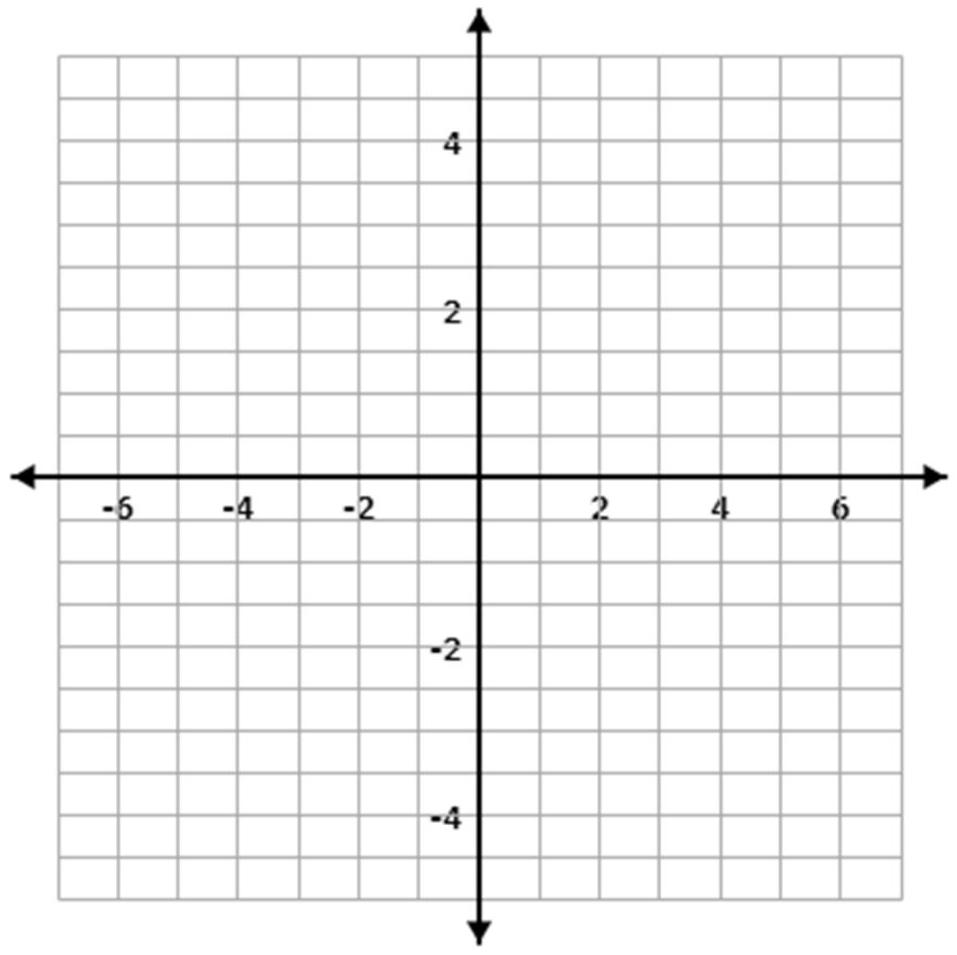
\includegraphics[max width=\textwidth, alt={}, center]{bb0c961a-4a4c-4f4a-bec0-1e84a1708d3c-16_955_957_1003_964}\\
c) Write the end behavior of $r(x)$ as $x$ decreases without bound as a limit statement (2 points)\\
d) Evaluate the 2 limits shown below (1 point each)

$$
\lim _{x \rightarrow-2^{+}} r(x)=\quad \lim _{x \rightarrow 1^{+}} r(x)=
$$

Simplify the expression (3 points)

$$
\frac{\frac{x-2}{4 x}}{\frac{x^{2}-4 x+4}{12 x}}
$$

Simplify the expression (3 points)

$$
\frac{\frac{1}{x}+8}{4-\frac{1}{x}}
$$

Find all real values of $x$ that satisfy the equation. Identify all algebraic solutions and indicate extraneous solutions by striking through them. (4 points)

$$
\frac{1}{x-4}-\frac{5}{x+2}=\frac{6}{x^{2}-2 x-8}
$$

Find all real values of $x$ that satisfy the equation. Identify all algebraic solutions and indicate extraneous solutions by striking through them. (5 points)

$$
\frac{2 x^{2}+5 x-5}{x-x^{2}}+\frac{1+x^{-1}}{1-x^{-1}}=\frac{1-x}{-x}
$$

\begin{enumerate}
  \item Let $h(x)=\frac{(x-2)(x+1)^{2}}{(x+1)(x-2)^{2}}$. Which of the following statements about the graph of $h$ is correct?\\
(A) The graph of $h$ has one hole and one vertical asymptote.\\
(B) The graph of $h$ has two holes and no vertical asymptotes.\\
(C) The graph of $h$ has no holes and two vertical asymptotes.\\
(D) The graph of $h$ has one hole and two vertical asymptotes.
  \item Let $h(x)=\frac{x^{3}+x^{2}-20 x}{x^{2}-8 x+16}$. Which of the following statements about the graph of $h$ is correct when $x=4$ ?\\
(A) The graph of $h$ only has a zero when $x=4$.\\
(B) The graph of $h$ only has a hole when $x=4$.\\
(C) The graph of $h$ only has a vertical asymptote when $x=4$.\\
(D) The graph of $h$ has both a zero and a vertical asymptote when $x=4$.
  \item The graph of the rational function $f$ has a hole at $x=5$ and a vertical asymptote at $x=-3$. Which of the following could be the expression for $f$ ?\\
(A) $\frac{(x-5)(x+2)}{(x-5)(x+3)}$\\
(B) $\frac{(x+2)(x+3)}{(x-5)(x+3)}$\\
(C) $\frac{(x-5)(x+3)}{(x-5)(x+2)}$\\
(D) $\frac{(x+5)(x+2)}{(x+5)(x-3)}$
  \item The graph of the rational function $h$ is shown below. Which of the following could be the expression for $h$ ?\\
(A) $\frac{(x-3)}{(x-3)(x-1)}$\\
(B) $\frac{(x+1)(x-3)}{(x-3)(x-1)}$\\
(C) $\frac{(x+1)(x-1)}{(x-3)(x-1)}$\\
(D) $\frac{(x-1)(x-3)}{(x-3)(x+1)}$\\
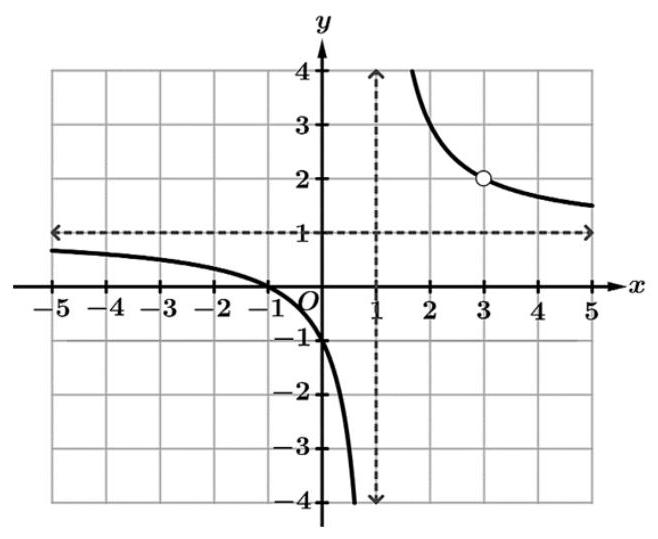
\includegraphics[max width=\textwidth, alt={}, center]{bb0c961a-4a4c-4f4a-bec0-1e84a1708d3c-20_539_658_216_1293}
  \item A rational function $r$ is given by $r(x)=\frac{x-2}{x+3}$. What are all intervals on which $r(x)>0$ ?\\
(A) $(-3,2)$\\
B) $(2, \infty)$\\
(C) $(-\infty,-3) \cup(2, \infty)$\\
(D) $(-\infty,-2) \cup(3, \infty)$
  \item If $\frac{12-6 x}{(x-1)(x+2)}=\frac{A}{x+2}+\frac{B}{x-1}$, what is the value of $B$ ?\\
(A) 2\\
(B) 8\\
(C) -2\\
(D) -8
  \item Let $g(x)=\frac{(x-2)^{2}(x+3)^{3}(x-4)^{2}}{(x-2)^{3}(x+3)^{2}}$. The graph of $g$ has a zeros at which of the following values of $x$ ?\\
(A) $x=4$ only\\
(B) $x=4$ and $x=-3$ only\\
(C) $x=2$ and $x=-3$ only\\
(D) $x=4, x=2$, and $x=-3$
\end{enumerate}

The graph of the rational function $f$ is shown below. Use the graph of $f$ to answer the following questions:\\
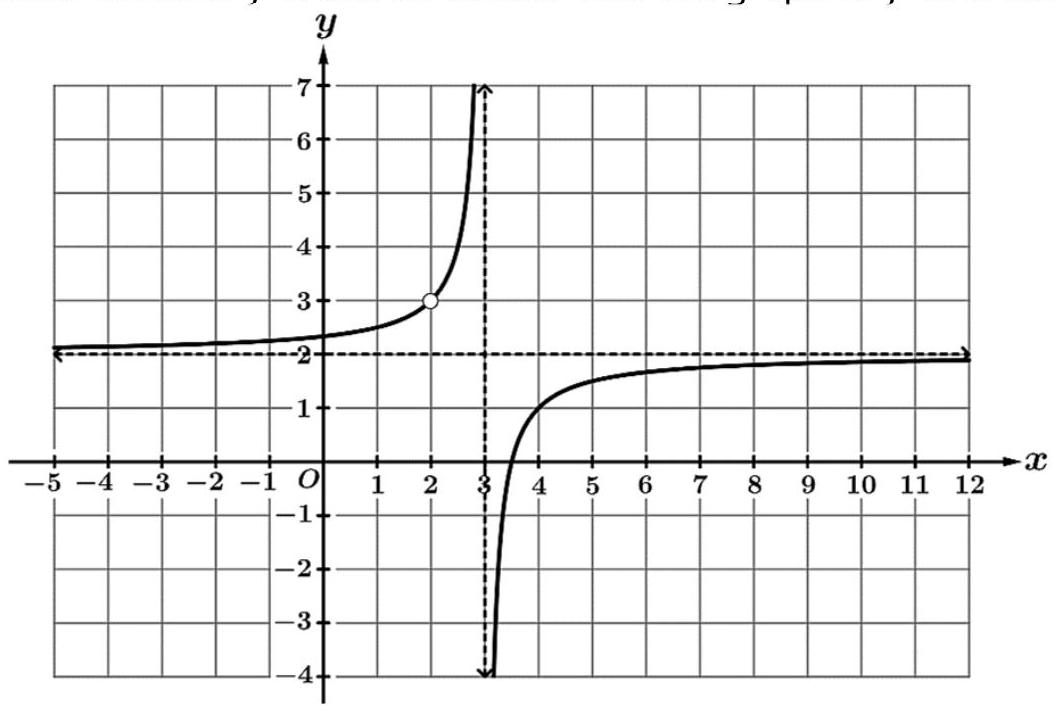
\includegraphics[max width=\textwidth, alt={}, center]{bb0c961a-4a4c-4f4a-bec0-1e84a1708d3c-21_717_1060_182_532}\\
8. $\lim _{x \rightarrow 2^{-}} f(x)=$\\
(A) 2\\
(B) 3\\
(C) $-\infty$\\
(D) $\infty$\\
9. $\lim _{x \rightarrow 3^{+}} f(x)=$\\
(A) 2\\
(B) 3\\
(C) $-\infty$\\
(D) $\infty$\\
10. $\lim _{x \rightarrow-\infty} f(x)=$\\
(A) 2\\
(B) 3\\
(C) $-\infty$\\
(D) $\infty$\\
11. Which of the following rational functions have a horizontal asymptote?\\
I. $f(x)=\frac{3 x^{2}+x-1}{x^{2}+4}$\\
II. $g(x)=\frac{(x+1)(2 x-3)^{2}}{(5 x-7)^{2}}$\\
III. $h(x)=\frac{x-4}{x^{3}+x^{2}-6}$\\
(A) I only\\
(B) I and II only\\
(C) I and III only\\
(D) I, II, and III\\
12. The graph of the rational function h has a horizontal asymptote of $y=-3$. Which of the following could be an expression for $h(x)$ ?\\
(A) $\frac{x^{2}-4 x+7}{-3 x^{2}+5}$\\
(B) $\frac{3 x^{2}-5 x-2}{x^{2}-x+1}$\\
(C) $\frac{-3 x^{3}+x-2}{x^{2}+5 x-6}$\\
(D) $\frac{-6 x^{3}+7 x^{2}-12}{2 x^{3}+11}$

Use the function $r(x)=\frac{4 x^{3}-12 x+8}{2 x^{3}+6 x^{2}-8}$ to answer the questions below.\\
a) Factor $r(x)$ and write it in a simplified form. Be sure to include domain restrictions (3 points)\\
b) Find the following key features of $r(x)$ (6 points). Then, sketch $r(x)$ on the axes provided (1 point)

\begin{center}
\begin{tabular}{|c|l|}
\hline
Domain &  \\
\hline
Vertical &  \\
Asymptote(s) &  \\
\hline
Horizontal &  \\
Asymptote(s) &  \\
\hline
Y-intercept(s) &  \\
\hline
X-intercept(s) &  \\
\hline
Hole(s) &  \\
\hline
\end{tabular}
\end{center}

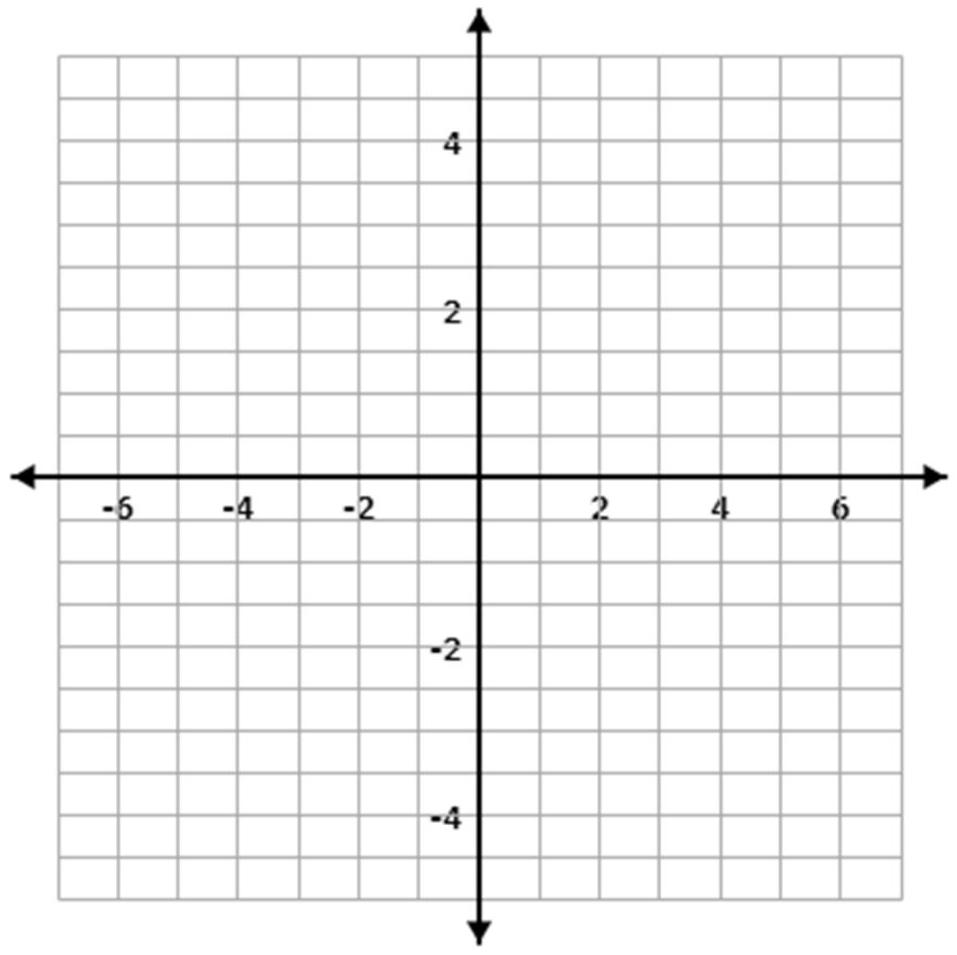
\includegraphics[max width=\textwidth, alt={}, center]{bb0c961a-4a4c-4f4a-bec0-1e84a1708d3c-22_955_957_1003_964}\\
c) Write the end behavior of $r(x)$ as $x$ decreases without bound as a limit statement (2 points)\\
d) Evaluate the 2 limits shown below (1 point each)

$$
\lim _{x \rightarrow-2^{+}} r(x)=\quad \lim _{x \rightarrow 1^{+}} r(x)=
$$

Simplify the expression (3 points)

$$
\frac{\frac{8 x}{x^{2}-1}}{\frac{10 x}{x+1}}
$$

Simplify the expression (3 points)

$$
\frac{4+\frac{1}{x^{2}}}{3-\frac{1}{x^{2}}}
$$

Find all real values of $x$ that satisfy the equation. Identify all algebraic solutions and indicate extraneous solutions by striking through them. (4 points)

$$
\frac{1}{x-3}-\frac{2}{x+1}=\frac{8}{x^{2}-2 x-3}
$$

Find all real values of $x$ that satisfy the equation. Identify all algebraic solutions and indicate extraneous solutions by striking through them. (5 points)

$$
\frac{3 x^{2}+2 x-3}{x-x^{2}}+\frac{1+x^{-1}}{1-x^{-1}}=\frac{1-x}{-x}
$$


\end{document}